\begin{frame}{Gestion des petits angles dans le cas 3D}

    \begin{figure}
        \centering
        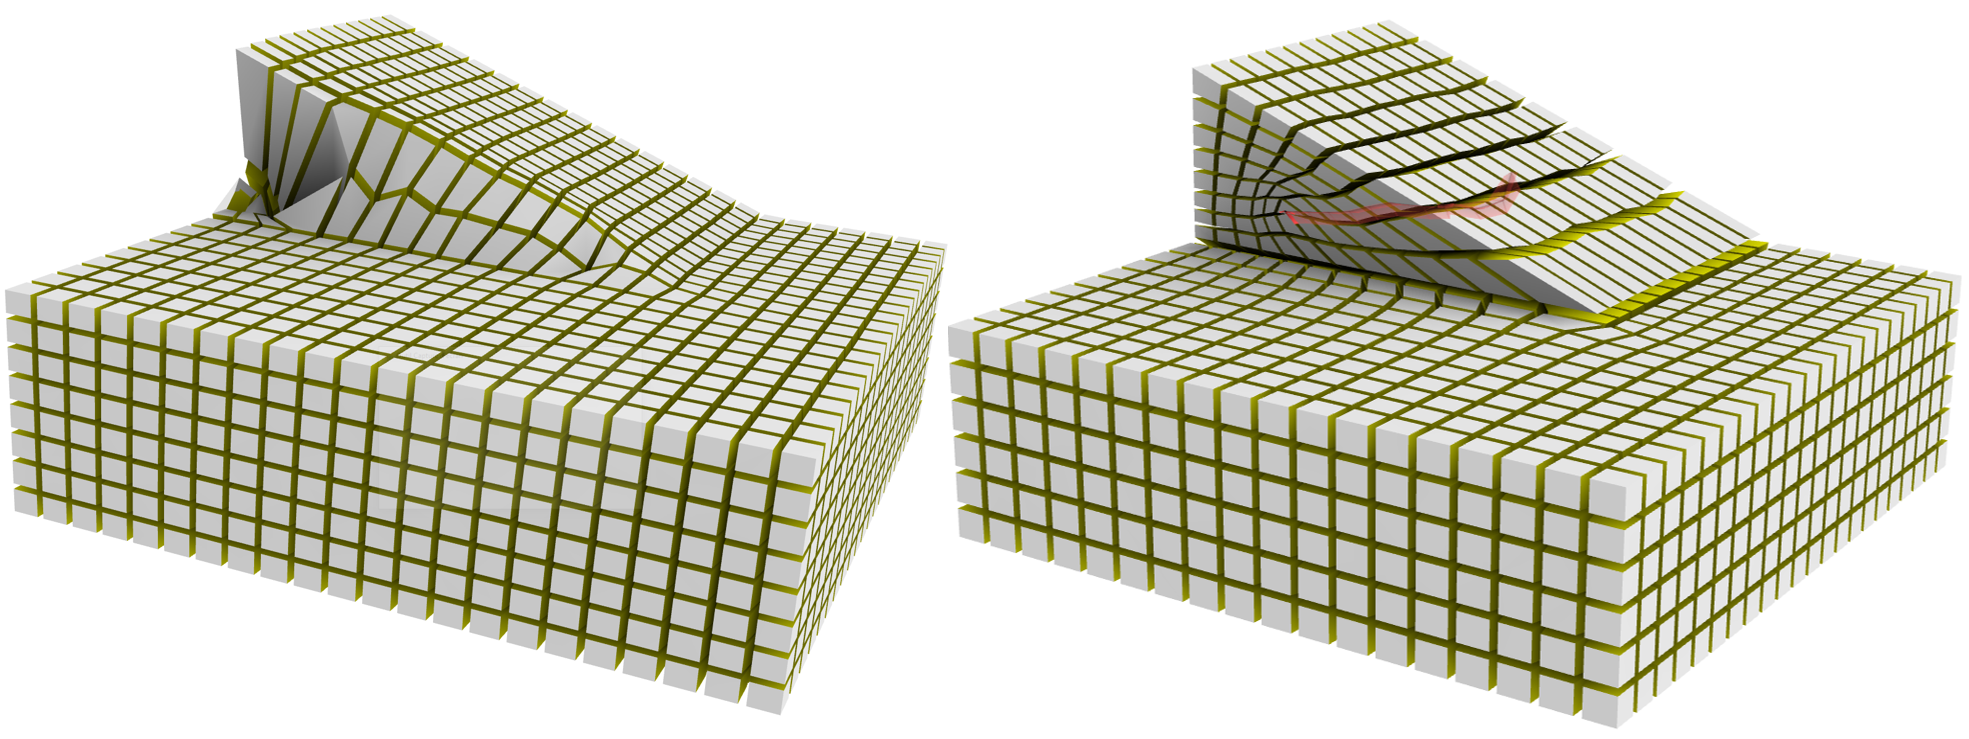
\includegraphics[width=0.99\textwidth]{img/hexmeshing_ff/tremplin_solved_2.PNG}
    \end{figure}
    
\end{frame}

\begin{frame}{Intuition de la méthode}

    \begin{figure}
        \centering
        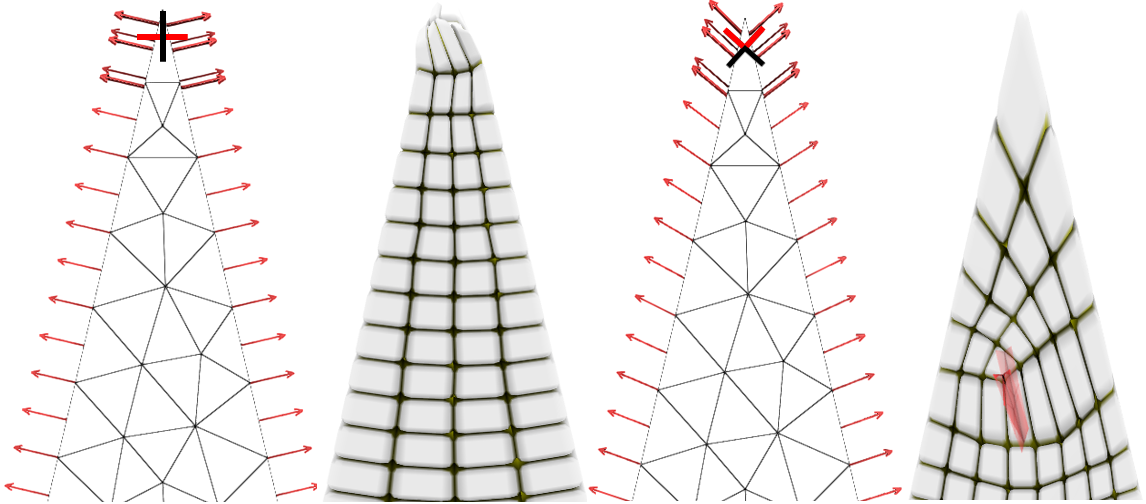
\includegraphics[width=0.99\textwidth]{img/hexmeshing_ff/normal_alignment_with_hexes_2.PNG}
    \end{figure}
    
\end{frame}

\begin{frame}{Calcul des angles dièdres et des valences géométriques}

    \begin{figure}
        \centering
        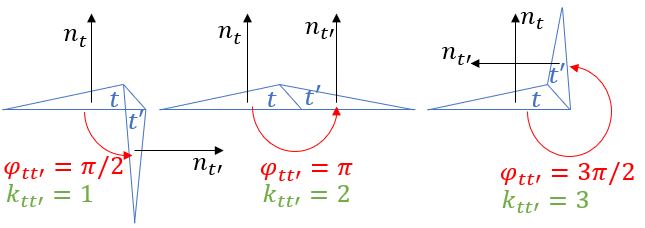
\includegraphics[width=0.8\textwidth]{img/hexmeshing_ff/phi_angles.PNG}
    \end{figure}
    
   
    \begin{align*}
        \varphi(n_t, n_{t'}) &= \pi - \mathrm{atan2} \left( \langle n_t \times n_{t'}, \frac{e_{tt'}}{\left|e_{tt'}\right|} \rangle, \langle n_t , n_{t'} \rangle \right)\\
        k_{tt'} &= \text{arrondi}( \frac{\varphi_{tt'}}{\pi/2} )
    \end{align*}
\end{frame}

\begin{frame}{Optimisation des normales de bord}

    \begin{align*}
        \delta_t^d(v) &= \max_{t' \in \mathcal{N}(t)} \left| \varphi( v_t, v_{t'} ) - k_{tt'}\pi/2 \right|\\
        \delta_t^n(v) &= \max_{t' \in \mathcal{N}(t)} \arccos\left( v_t^\top \bar{n}_{tt'}\right)\\
        \mathcal{E}(v) &= \max_{t \in V_b} \max (\delta_t^d(v), \delta_t^n(v) )
    \end{align*} 
    L'objectif est de trouver le champ de vecteurs $v$ qui minimise $\mathcal{E}(v)$.
    
\end{frame}

\begin{frame}{Recherche du vecteur $v_t$ minimisant $\mathcal{E}_t(v)$ }

    \begin{figure}
        \centering
        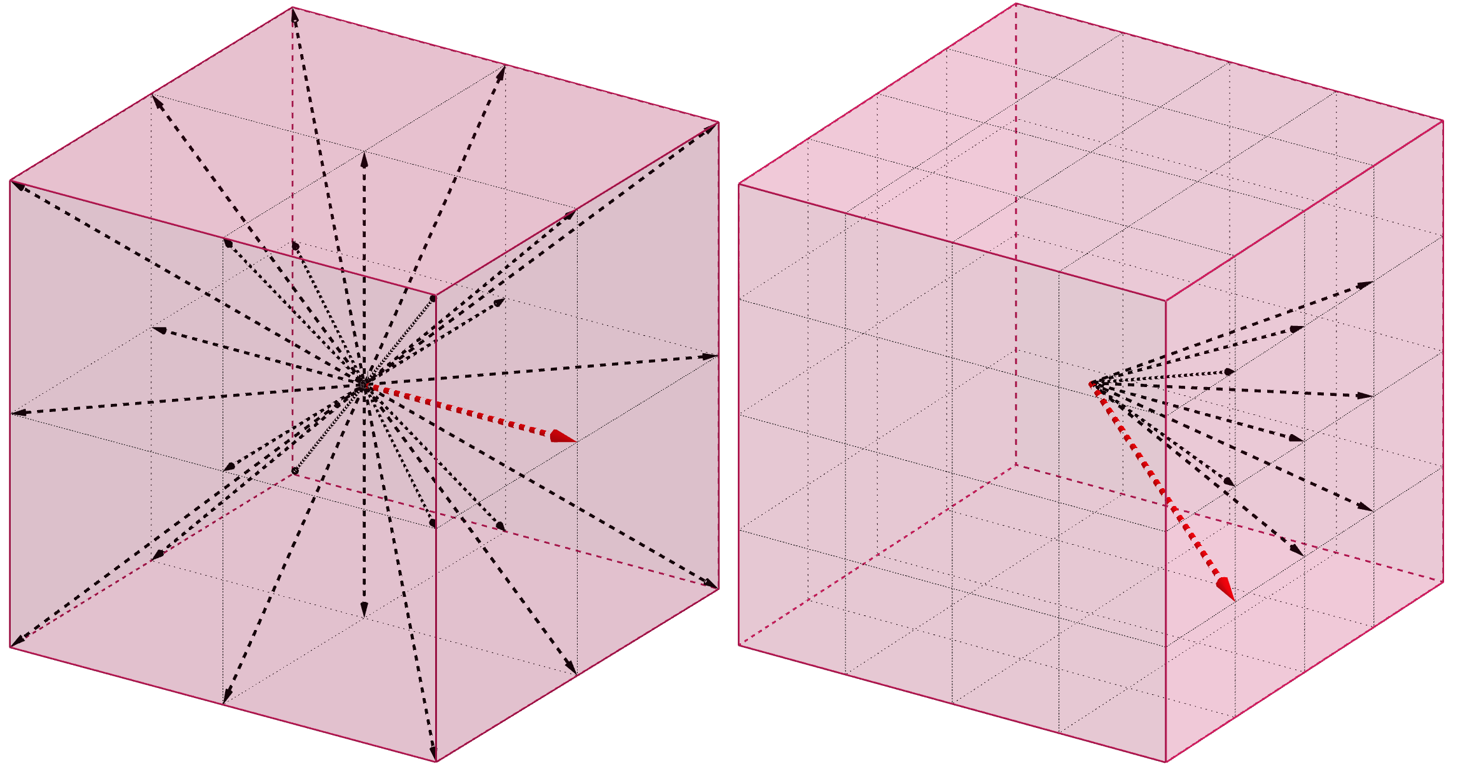
\includegraphics[width=0.99\textwidth]{img/hexmeshing_ff/finding_directions_in_a_cube_2.PNG}
    \end{figure}
\end{frame}

\begin{frame}{Algorithme glouton pour calculer le champ de vecteur de bord}

    \begin{center}
        \begin{minipage}{0.4\linewidth}
        \end{minipage}
        \begin{minipage}{0.59\linewidth}
            \begin{algorithm}[H]
                \small
                \SetAlgoLined
                \label{algo:iterative_constraints}
                \SetKwProg{Fn}{Function}{:}{}
                \Fn{IterativeOptimization(n)}{
                $v \gets n$\\%initial normal vectors of boundary facets;
                $Q \gets$ boundary facet indices;\\
                \While{$Q$ is not empty}{
                $i \gets Q$.pop\_front();\\
                ${u} \gets$ MinFacetDirection($i$);\\
                \If{$\mathcal{E}(u) < \mathcal{E}(v)$}{
                ${v_t} \gets u_t$;\\
                \ForAll{$t' \in \mathcal{N}(t)$}{
                $Q$.push($j$);
                }
                }
                }
                \Return{$v$};
                }

            \end{algorithm}
        \end{minipage}
    \end{center}
\end{frame}        




\begin{frame}{Différentes stratégies pour déterminer $k_{tt'}$:\\ Empêcher la valeur $k_{tt'} = 0$}
    \begin{figure}
        \centering
        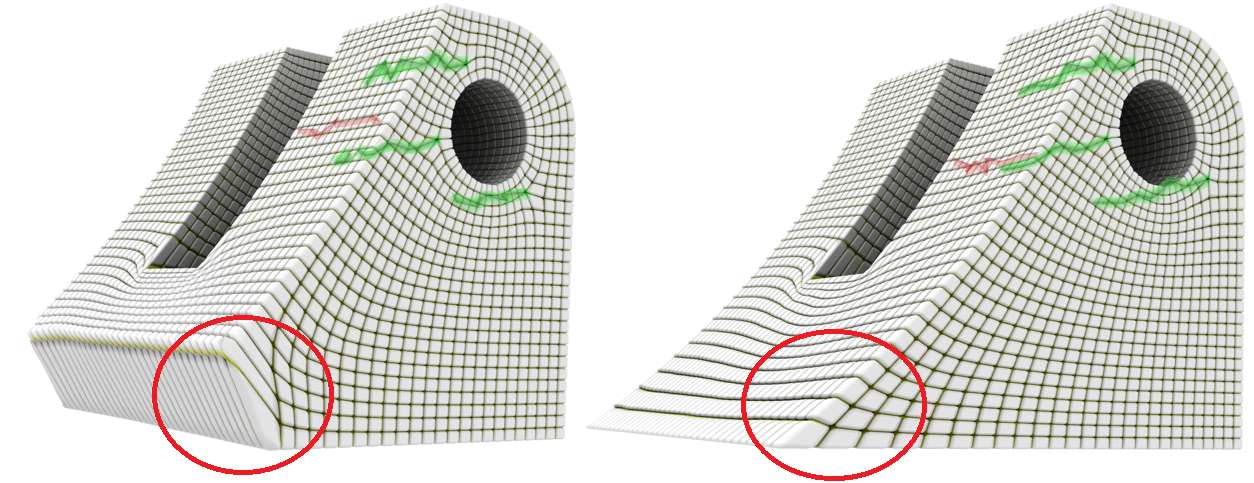
\includegraphics[width=\textwidth]{img/hexmeshing_ff/comparison_low_angle_edge_2.PNG}
    \end{figure}
\end{frame}

\iffalse
\begin{frame}{Différentes stratégies pour déterminer $k_{tt'}$:\\Angles diédraux ambigus}
    \begin{figure}
        \centering
        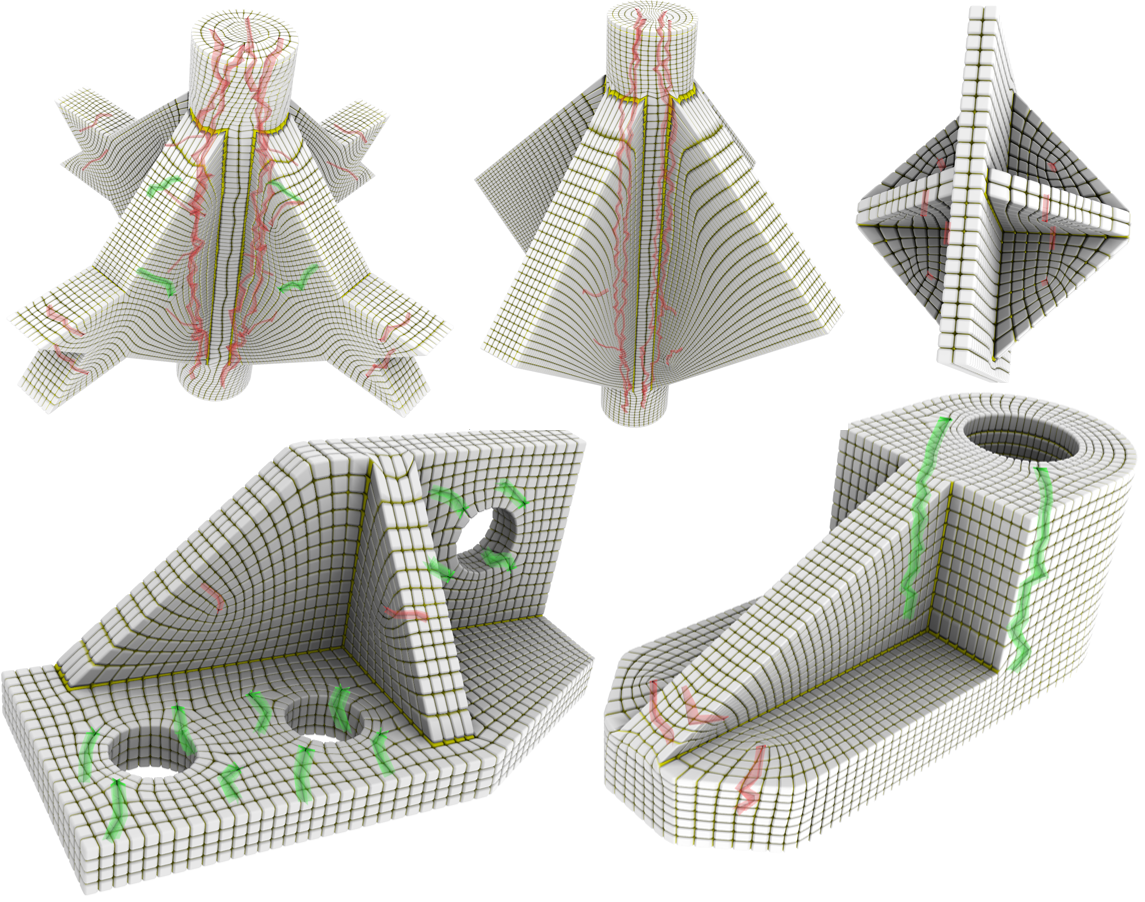
\includegraphics[width=0.75\textwidth]{img/hexmeshing_ff/resultats_3.png}
    \end{figure}
\end{frame}
\fi
\begin{frame}{Différentes stratégies pour déterminer $k_{tt'}$:\\Valences prescrites dans des modèles CAO}

    \begin{figure}
        \centering
        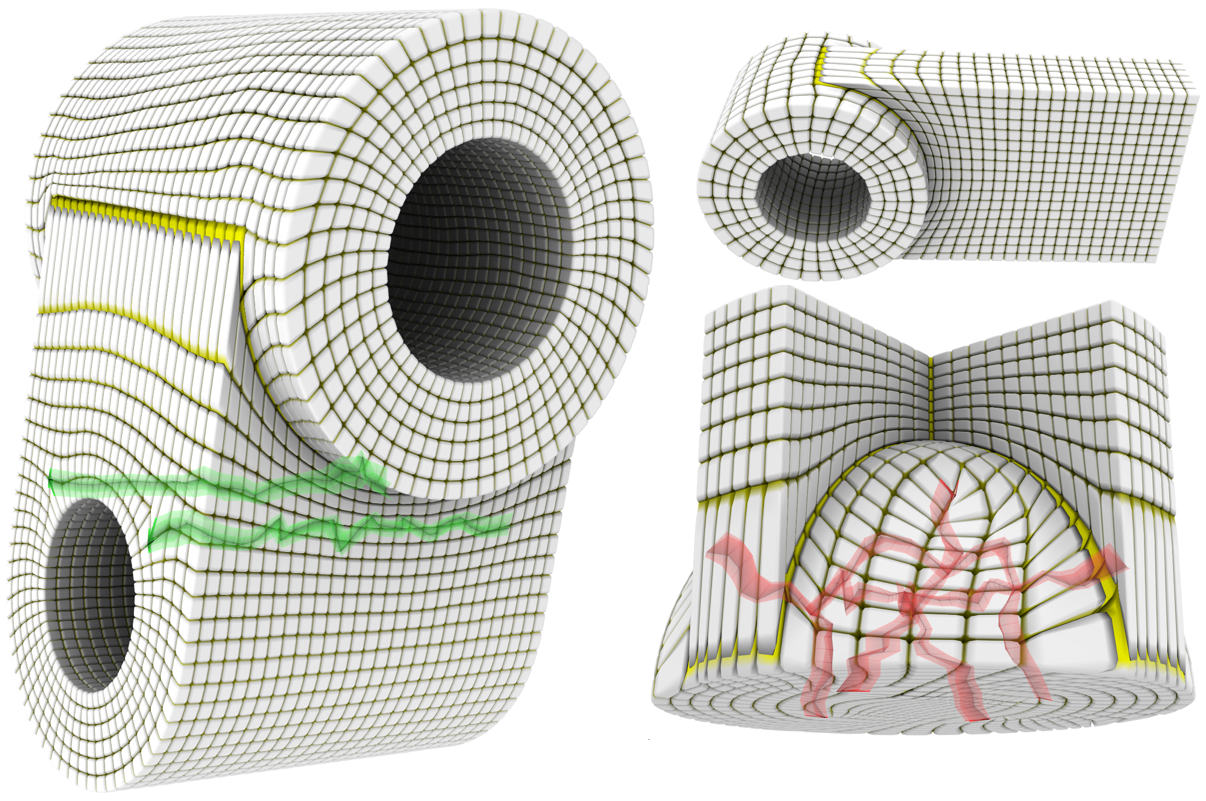
\includegraphics[width=0.9\textwidth]{img/hexmeshing_ff/prescribed_valences.PNG}
    \end{figure}
    
\end{frame}

\begin{frame}{Maillage hexaédrique avec valence d'arête supérieure à 4}
    \begin{figure}
        \centering
        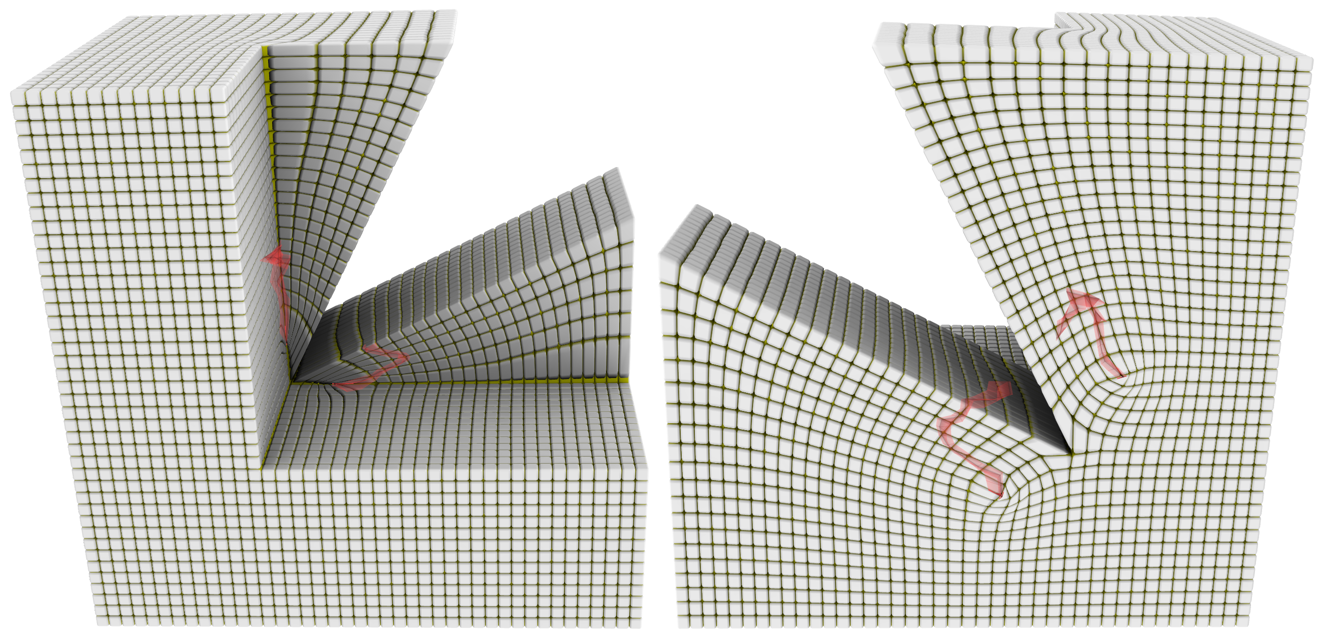
\includegraphics[width=0.99\textwidth]{img/hexmeshing_ff/valence_5_edges.PNG}
    \end{figure}
\end{frame}